\section{The Module Graph}
\label{sec:module-import}

We begin with the coarsest level of analysis: module-level structures. Two graphs on the same vertex set $\mathcal{M}$ (the set of all \module{Mathlib} modules) capture complementary aspects of the library's organization. The \emph{module tree} $T$ (\S\ref{sec:module-names}--\S\ref{sec:namespace-tree}) inherits the cognitive classification that mathematicians have long applied to their subject. The \emph{module graph} $G_{\mathrm{module}}$ (\S\ref{sec:import-graph}) records the logical dependencies enforced by the compiler. Throughout this section, $T$ serves as the cognitive baseline against which we measure the structure of $G_{\mathrm{module}}$.

\subsection{Modules}
\label{sec:module-names}
\begin{definition}[Module]\label{def:module}
A \emph{module} in \module{Mathlib} is identified by a dot-separated sequence of identifiers, such as $\module{Mathlib.Algebra.Group.Defs}$. Each module corresponds to a \texttt{.lean} source file, with dots replacing path separators. We write $\mathcal{M}$ for the set of all modules in \module{Mathlib}:
\begin{align*}
  \mathcal{M} = \{\; &\module{Mathlib.Init},\\
    &\module{Mathlib.Algebra.Group.Defs},\\
    &\module{Mathlib.Analysis.Normed.Group.Basic},\; \ldots\,\}.
\end{align*}
The \emph{depth} of a module $c_1.c_2.\cdots.c_k$ is~$k$, the number of dot-separated components.
\end{definition}

All statistics in this paper are computed from commit \texttt{534cf0b} (2 February 2026) of the \module{Mathlib} repository, using the official \texttt{importGraph} tool~\cite{importgraph}. At this commit, $|\mathcal{M}| = 7{,}563$. The set $\mathcal{M}$ serves as the shared vertex set for both graphs defined in this section.

\begin{example}
\leavevmode
\begin{itemize}
  \item $\module{Mathlib}$ has depth~$1$.
  \item $\module{Mathlib.Algebra}$ has depth~$2$.
  \item $\module{Mathlib.Algebra.Group.Defs}$ has depth~$4$.
\end{itemize}
The maximum depth in \module{Mathlib} is~$7$.\footnote{Attained by, e.g., \module{Mathlib.CategoryTheory.Limits.Shapes.Pullback.IsPullback.Kernels}.}
\end{example}

\subsection{The Module Hierarchy}
\label{sec:namespace-tree}

Modules are organized hierarchically: each dot-separated name mirrors a path in the source repository.

\begin{figure}[H]
\centering
\begin{subfigure}[t]{0.42\textwidth}
\centering
\begin{forest}
  for tree={
    font=\scriptsize\ttfamily,
    grow'=0,
    child anchor=west,
    parent anchor=south,
    anchor=west,
    calign=first,
    edge path={
      \noexpand\path [draw, \forestoption{edge}]
        (!u.south west) +(7.5pt,0) |- (.child anchor)\forestoption{edge label};
    },
    before typesetting nodes={
      if n=1 {insert before={[,phantom]}} {}
    },
    fit=band,
    before computing xy={l=13pt},
  }
[Mathlib/
  [Algebra/
    [Group/
      [Defs.lean]
    ]
  ]
  [Data/
    [Nat/
      [Notation.lean]
    ]
  ]
  [\ldots, edge={draw, densely dotted}]
]
\end{forest}
\caption{Directory structure}
\label{fig:dir-tree}
\end{subfigure}%
\hfill
\begin{subfigure}[t]{0.52\textwidth}
\centering
\begin{tikzpicture}[
  every node/.style={font=\scriptsize\ttfamily, inner sep=2pt, text=blue!60!black},
  dot/.style={circle, fill=blue!60!black, minimum size=3pt, inner sep=0pt},
  dep/.style={->, >=Stealth, thin, blue!60!black},
]
  \node[dot, label=above:{Mathlib}]              (root) at (1.8,0) {};
  \node[dot, label=left:{Algebra}]               (alg)  at (0,-1.3) {};
  \node[dot, label=right:{Data}]                 (dat)  at (3.6,-1.3) {};
  \node[dot, label=left:{Algebra.Group}]         (grp)  at (0,-2.6) {};
  \node[dot, label=right:{Data.Nat}]             (nat)  at (3.6,-2.6) {};
  \node[dot, label=below:{Algebra.Group.Defs}]   (gd)   at (0,-3.9) {};
  \node[dot, label=below:{Data.Nat.Notation}]    (nn)   at (3.6,-3.9) {};
  \draw[dep] (root) -- (alg);
  \draw[dep] (root) -- (dat);
  \draw[dep] (alg)  -- (grp);
  \draw[dep] (dat)  -- (nat);
  \draw[dep] (grp)  -- (gd);
  \draw[dep] (nat)  -- (nn);
  \node[font=\scriptsize, text=gray] at (1.8,-1.3) {$\cdots$};
\end{tikzpicture}
\caption{Module tree $T$: arrows point parent $\to$ child ($\in E_T$)}
\label{fig:namespace-tree}
\end{subfigure}
\caption{A fragment of the \module{Mathlib} source tree (commit \texttt{534cf0b}). Left: the directory layout. Right: the corresponding rooted tree~$T$. Each directory path maps to a module with dots replacing separators, e.g., \module{Mathlib/\allowbreak Algebra/\allowbreak Group/\allowbreak Defs.lean} $\leftrightarrow$ \module{Mathlib.\allowbreak Algebra.\allowbreak Group.\allowbreak Defs}.}
\label{fig:prefix-tree}
\end{figure}

We say $m$ is a \emph{prefix} of $m'$ if $m'$ extends $m$ by additional components. For example, \module{Mathlib.Algebra} is a prefix of \module{Mathlib.Algebra.Group.Defs}.

\begin{definition}[Module tree]\label{def:module-tree}
The prefix relation induces a rooted tree $T = (\mathcal{M}, E_T)$ with root $\module{Mathlib}$, which we call the \emph{module tree}, where
\[
  E_T = \{(m, m') \in \mathcal{M} \times \mathcal{M} \mid m \text{ is a prefix of } m' \text{ and } \mathrm{depth}(m') = \mathrm{depth}(m) + 1\}.
\]
Its leaves are modules (source files); its internal nodes are shared prefixes of modules, corresponding to directories in the source repository.
\end{definition} This hierarchy is distinct from Lean~4's \texttt{namespace} mechanism: in Lean~4, the \texttt{namespace} keyword creates a naming scope that need not align with file boundaries---a single namespace may span many files, and a single file may contribute declarations to multiple namespaces (\S\ref{sec:ns-mod-cross}). The two often coincide in practice, since \module{Mathlib}'s top-level directories (\module{Algebra}, \module{Analysis}, \module{CategoryTheory}, etc.) serve as both directory names and the primary organizational categories.

The top-level directories (children of the root) include \module{Algebra} (1257 files), \module{CategoryTheory} (982 files), \module{Analysis} (755 files), etc.

\subsection{The Module Graph}
\label{sec:import-graph}

Each Lean source file begins with \texttt{import} statements that declare its dependencies. For example, the file \module{Mathlib/Data/Nat/Notation.lean} contains:

\begin{codebox}
\textsf{\bfseries\color{blue!60!black}Data/Nat/Notation.lean}\\[2pt]
\textbf{public import} \textcolor{blue!60!black}{Mathlib.Init}
\end{codebox}

\noindent
This file depends on exactly one other module: \module{Mathlib.Init}.

A file with more dependencies is \module{Mathlib/Algebra/Group/Defs.lean}, which imports nine modules (shown here in abbreviated form):

\begin{codebox}
\textsf{\bfseries\color{blue!60!black}Algebra/Group/Defs.lean}\\[2pt]
\textbf{public import} \textcolor{blue!60!black}{Batteries.Logic}\\
\textbf{public import} \textcolor{blue!60!black}{Mathlib.Algebra.Notation.Defs}\\
\textbf{public import} \textcolor{blue!60!black}{Mathlib.Algebra.Regular.Defs}\\
\hspace{1.5em}\textit{\color{gray}-- \ldots\ 6 more imports}
\end{codebox}

\noindent
Each file is a \emph{vertex} in the module graph; each \texttt{import} statement is a directed \emph{edge} from the importing module to the imported module.

Lean~4 supports both \texttt{import} and \texttt{public import}; the latter re-exports the imported module to downstream dependents. For the purposes of the module graph, both forms create an edge---they differ only in visibility, not in the dependency relationship.

\begin{definition}[Import set]
For each $m \in \mathcal{M}$, let $\mathrm{imports}(m) \subseteq \mathcal{M}$ denote the set of modules directly imported by $m$ (via either \texttt{import} or \texttt{public import}).
\end{definition}

\begin{definition}[Module graph]
The \emph{module graph} of \module{Mathlib} is $G_{\mathrm{module}} = (\mathcal{M}, E_{\mathrm{module}})$ where
\[
  E_{\mathrm{module}} = \{(m_1, m_2) \in \mathcal{M} \times \mathcal{M} \mid m_2 \in \mathrm{imports}(m_1)\}.
\]
\end{definition}

Since \module{Mathlib/Data/Nat/Notation.lean} contains \texttt{public import Mathlib.Init}, we have the edge $(\module{Data.Nat.Notation},\; \module{Init}) \in E_{\mathrm{module}}$:

\begin{figure}[H]
\centering
\begin{tikzpicture}[
  every node/.style={font=\small\ttfamily, inner sep=2pt, text=blue!60!black},
  dot/.style={circle, fill=blue!60!black, minimum size=3pt, inner sep=0pt},
  dep/.style={->, >=Stealth, thin, blue!60!black},
]
  \node[dot, label=above:{Init}]              (b) at (0,0) {};
  \node[dot, label=above:{Data.Nat.Notation}] (a) at (4,0) {};
  \draw[dep] (a) -- (b);
\end{tikzpicture}
\caption{The simplest import edge: \module{Data.Nat.Notation} imports \module{Init}. The arrow points from the importing module to the imported module. All names have the \module{Mathlib.}\ prefix removed.}
\label{fig:single-import-edge}
\end{figure}

\begin{remark}
The module tree $T$ and the module graph $G_{\mathrm{module}}$ are distinct structures on the same vertex set $\mathcal{M}$. In $T$, edges connect a module to its prefix parent in the directory hierarchy; in $G_{\mathrm{module}}$, edges reflect explicit \texttt{import} dependencies. Import edges need not respect the directory hierarchy.
\end{remark}

The contrast between these two structures is conceptually significant. The module tree $T$ encodes a \emph{cognitive} organization of mathematics: its top-level directories---\module{Algebra}, \module{Analysis}, \module{Topology}---reflect a classification that mathematicians established long before formalization. The module graph $G_{\mathrm{module}}$, by contrast, encodes \emph{logical} dependencies that need not respect this classification. The extent to which $G_{\mathrm{module}}$ deviates from $T$---edges that cross directory boundaries, dependencies that link distant branches of the tree---reveals the internal structure of mathematics that no human taxonomy fully captures.

\begin{figure}[ht]
\centering
\begin{tikzpicture}[
  every node/.style={font=\small\ttfamily, inner sep=2pt, text=blue!60!black},
  dot/.style={circle, fill=blue!60!black, minimum size=3pt, inner sep=0pt},
  dep/.style={->, >=Stealth, thin, blue!60!black},
]
  \node[dot, label=above:{Init}]                (d) at (0,0) {};
  \node[dot, label=left:{Data.Int.Notation}]    (b) at (-1.5,-1.5) {};
  \node[dot, label=right:{Data.Nat.Notation}]   (c) at (1.5,-1.5) {};
  \node[dot, label=below:{Algebra.Group.Defs}]  (a) at (0,-3) {};

  \draw[dep] (a) -- (b);
  \draw[dep] (a) -- (c);
  \draw[dep] (b) -- (d);
  \draw[dep] (c) -- (d);
\end{tikzpicture}
\caption{A fragment of $G_{\mathrm{module}}$: \module{Algebra.Group.Defs} imports two modules that both depend on \module{Init}, forming a diamond. All names have the \module{Mathlib.}\ prefix removed.}
\label{fig:import-subgraph}
\end{figure}

The module graph $G_{\mathrm{module}}$ is DAG: we verified this by computing a topological ordering of all $7{,}563$ modules using the \texttt{importGraph} tool~\cite{importgraph}.\footnote{The \texttt{importGraph} tool outputs edges in the reverse direction (imported $\to$ importing). Our definition follows the standard dependency convention (importing $\to$ imported); acyclicity is invariant under edge reversal.} 

\subsection{Transitive Reduction and Redundant Imports}
\label{sec:transitive-reduction}

Since $G_{\mathrm{module}}$ is a DAG, it has a unique \emph{transitive reduction}~\cite{ahu1972}: the smallest subgraph $G_{\mathrm{module}}^{-} \subseteq G_{\mathrm{module}}$ with the same reachability relation. An edge $(m_1, m_2) \in E_{\mathrm{module}}$ is \emph{transitively redundant} if $m_2$ is reachable from $m_1$ via a path of length $\ge 2$ in $G_{\mathrm{module}}$---that is, the dependency is already implied by other imports.

\begin{definition}[Transitive reduction]
The \emph{transitive reduction} of $G_{\mathrm{module}}$ is $G_{\mathrm{module}}^{-} = (\mathcal{M}, E_{\mathrm{module}}^{-})$ where
\[
  E_{\mathrm{module}}^{-} = E_{\mathrm{module}} \setminus \{(m_1, m_2)\in E_{\mathrm{module}} \mid \exists\, \text{path } m_1 \to \cdots \to m_2 \text{ in } G_{\mathrm{module}} \text{ of length} \ge 2\}.
\]
\end{definition}

\begin{figure}[H]
\centering
\begin{subfigure}[t]{0.42\textwidth}
\centering
\vspace{0pt}
\begin{tikzpicture}[
  every node/.style={font=\scriptsize\ttfamily, inner sep=1pt, text=blue!60!black},
  dot/.style={circle, fill=blue!60!black, minimum size=3pt, inner sep=0pt},
  dep/.style={->, >=Stealth, thin, blue!60!black},
  redundant/.style={->, >=Stealth, orange!80!red, dashed, thick},
]
  \node[dot, label=above:{Init}]                (d) at (0,0) {};
  \node[dot, label=left:{Data.Int.Notation}]    (b) at (-1.2,-1.2) {};
  \node[dot, label=right:{Data.Nat.Notation}]   (c) at (1.2,-1.2) {};
  \node[dot, label=below:{Algebra.Group.Defs}]  (a) at (0,-2.4) {};

  \draw[dep] (a) -- (b);
  \draw[dep] (a) -- (c);
  \draw[dep] (b) -- (d);
  \draw[dep] (c) -- (d);
  \draw[redundant] (a) -- (d);
\end{tikzpicture}
\caption{Subgraph of $G_{\mathrm{module}}$}
\label{fig:tr-graph}
\end{subfigure}%
\hfill
\begin{subfigure}[t]{0.46\textwidth}
\vspace{0pt}\raggedleft
\scriptsize\ttfamily
\begin{tabular}[t]{@{}l@{}}
  \textnormal{\sffamily\bfseries\color{blue!60!black} Data/Int/Notation.lean} \\[1pt]
  \hspace{1em}public import \textcolor{blue!60!black}{Init} \\[6pt]
  \textnormal{\sffamily\bfseries\color{blue!60!black} Data/Nat/Notation.lean} \\[1pt]
  \hspace{1em}public import \textcolor{blue!60!black}{Init} \\[6pt]
  \textnormal{\sffamily\bfseries\color{blue!60!black} Algebra/Group/Defs.lean} \\[1pt]
  \hspace{1em}public import \textcolor{blue!60!black}{Data.Int.Notation} \\
  \hspace{1em}public import \textcolor{blue!60!black}{Data.Nat.Notation} \\
  \hspace{1em}\textcolor{orange!80!red}{public import \textcolor{blue!60!black}{Init}}
    \textnormal{\sffamily\color{orange!80!red} $\leftarrow$ would be redundant} \\
\end{tabular}
\caption{Source file headers}
\label{fig:tr-source}
\end{subfigure}
\caption{Illustrating transitive redundancy on the diamond from Figure~\ref{fig:import-subgraph}. If \module{Algebra.Group.Defs} were to import \module{Init} directly (\textcolor{orange!80!red}{dashed orange} edge), that edge would be transitively redundant: \module{Init} is already reachable via both \module{Data.Int.Notation} and \module{Data.Nat.Notation}. All names have the \module{Mathlib.}\ prefix removed.}
\label{fig:transitive-reduction}
\end{figure}

The raw module graph has $|E_{\mathrm{module}}| = 23{,}570$ edges. After transitive reduction, $|E_{\mathrm{module}}^{-}| = 19{,}448$ edges, removing $4{,}122$ redundant edges ($17.5\%$). These redundant imports are syntactically present in the source files but logically unnecessary: the Lean compiler resolves them through transitive dependencies regardless. These redundant edges are not accidents of careless coding. Developers deliberately import umbrella modules---such as importing all of group theory rather than a single lemma---to maintain a navigable mental model of the library. The redundancy reflects a cognitive need: the gap between what the compiler requires and what the human reader requires to understand a file's mathematical context.

The \texttt{importGraph} tool applies transitive reduction by default when generating its output. We verified (via our own parser) that its reduced graph ($20{,}881$ edges including the umbrella root \module{Mathlib}) agrees exactly with our independently computed reduction on the shared $7{,}563$ modules: all $19{,}448$ edges in $G_{\mathrm{module}}^{-}$ appear in the tool's output, and the $1{,}433$ additional edges in the tool's output are precisely the edges from the umbrella module \module{Mathlib} to its direct children.

\subsection{Module Containment Decay}
\label{sec:module-containment}

The module graph's relationship to the module hierarchy $T$ can be quantified at every depth of the hierarchy, not only at the top level. At each depth~$k$, we truncate both endpoints of every import edge to their first~$k$ dot-separated components and measure the proportion of edges whose truncated endpoints match.

\begin{definition}[Module containment at depth~$k$]
\label{def:module-containment}
For each depth $k \ge 1$, let $\mathrm{trunc}_k(m)$ denote the first~$k$ components of module~$m$. The \emph{module containment ratio at depth~$k$} is
\[
  \mathrm{contain}_{\mathrm{mod}}(k) \;=\; \frac{|\{(m_1,m_2) \in E_{\mathrm{module}} \mid \mathrm{trunc}_k(m_1) = \mathrm{trunc}_k(m_2)\}|}{|E_{\mathrm{module}}|}.
\]
\end{definition}

Module depth is concentrated: $55.7\%$ of modules have depth~$4$ (e.g., \module{Mathlib.Data.Nat.Basic}), with a mean of~$4.22$ and a maximum of~$7$. Table~\ref{tab:module-containment} reports containment at each depth.

\begin{table}[ht]
\centering
\caption{Module-level containment decay by module depth. At depth~$1$ ($13$ top-level packages), $97.5\%$ of import edges stay within the same package; by depth~$4$, containment has fallen to~$8.8\%$.}
\label{tab:module-containment}
\begin{tabular}{crrr}
\toprule
Depth $k$ & Groups & Containment & $\Delta$ (pp) \\
\midrule
$1$ & $13$      & $97.5\%$  & ---     \\
$2$ & $99$      & $60.2\%$  & $-37.3$ \\
$3$ & $1{,}481$ & $34.1\%$  & $-26.1$ \\
$4$ & $5{,}641$ & $8.8\%$   & $-25.3$ \\
$5$ & $7{,}434$ & $0.8\%$   & $-8.0$  \\
\bottomrule
\end{tabular}
\end{table}

At depth~$1$, the $13$ top-level packages (\module{Mathlib}, \module{Batteries}, \module{Init}, etc.) contain $97.5\%$ of all import edges---nearly all imports stay within \module{Mathlib}. The steepest single drop occurs at depth~$1 \to 2$ ($-37.3$ pp), when packages split into their subdirectories: \module{Mathlib} divides into \module{Mathlib.Algebra}, \module{Mathlib.Analysis}, \module{Mathlib.CategoryTheory}, etc. The $60.2\%$ containment at depth~$2$ is consistent with the $61.4\%$ intra-directory rate reported below (\S\ref{sec:cross-namespace}), since depth-$2$ groups correspond precisely to the top-level directories under \module{Mathlib/}.\footnote{The small discrepancy ($60.2\%$ vs.\ $61.4\%$) reflects a difference in edge counts between our import parser and the \texttt{importGraph} tool.} By depth~$4$---the modal depth of modules---containment has fallen to $8.8\%$, and by depth~$5$ it is negligible.

The steep collapse reveals that, within a discipline, dependencies routinely cross subdirectory boundaries. A file in \module{Mathlib.Algebra.Group} may import from \module{Mathlib.Algebra.Ring} or \module{Mathlib.Algebra.Order}---directories that the hierarchy treats as siblings but that are tightly coupled mathematically. The containment curve for declaration-level dependencies, measured in \S\ref{sec:containment-decay}, starts from a much lower baseline ($48.9\%$ at the top-level directory) but exhibits the same qualitative pattern of steep initial decline and rapid saturation. The gap between the two baselines quantifies how effectively the module graph compresses cross-cutting declaration-level dependencies into within-discipline edges.

\subsection{Cross-Directory Dependencies}
\label{sec:cross-namespace}

\begin{definition}[Top-level directory]
For a module $m = \module{Mathlib.}X.Y.\cdots$, the \emph{top-level directory} is $\mathrm{dir}(m) = X$, the first directory component under the \module{Mathlib/} root.
\end{definition}

An edge $(m_1, m_2) \in E_{\mathrm{module}}$ is \emph{intra-directory} if $\mathrm{dir}(m_1) = \mathrm{dir}(m_2)$ and \emph{inter-directory} otherwise. In $G_{\mathrm{module}}$, $14{,}464$ edges ($61.4\%$) are intra-directory and $9{,}106$ ($38.6\%$) are inter-directory. In $G_{\mathrm{module}}^{-}$, the proportions are similar: $12{,}226$ ($62.9\%$) intra and $7{,}222$ ($37.1\%$) inter.

If the module graph perfectly respected the directory hierarchy---that is, if every module only depended on modules within its own top-level directory---the heatmap below would be purely diagonal. Each off-diagonal bright cell therefore represents a point where the logical structure of proofs departs from the cognitive classification of~$T$.

\begin{figure}[H]
\centering
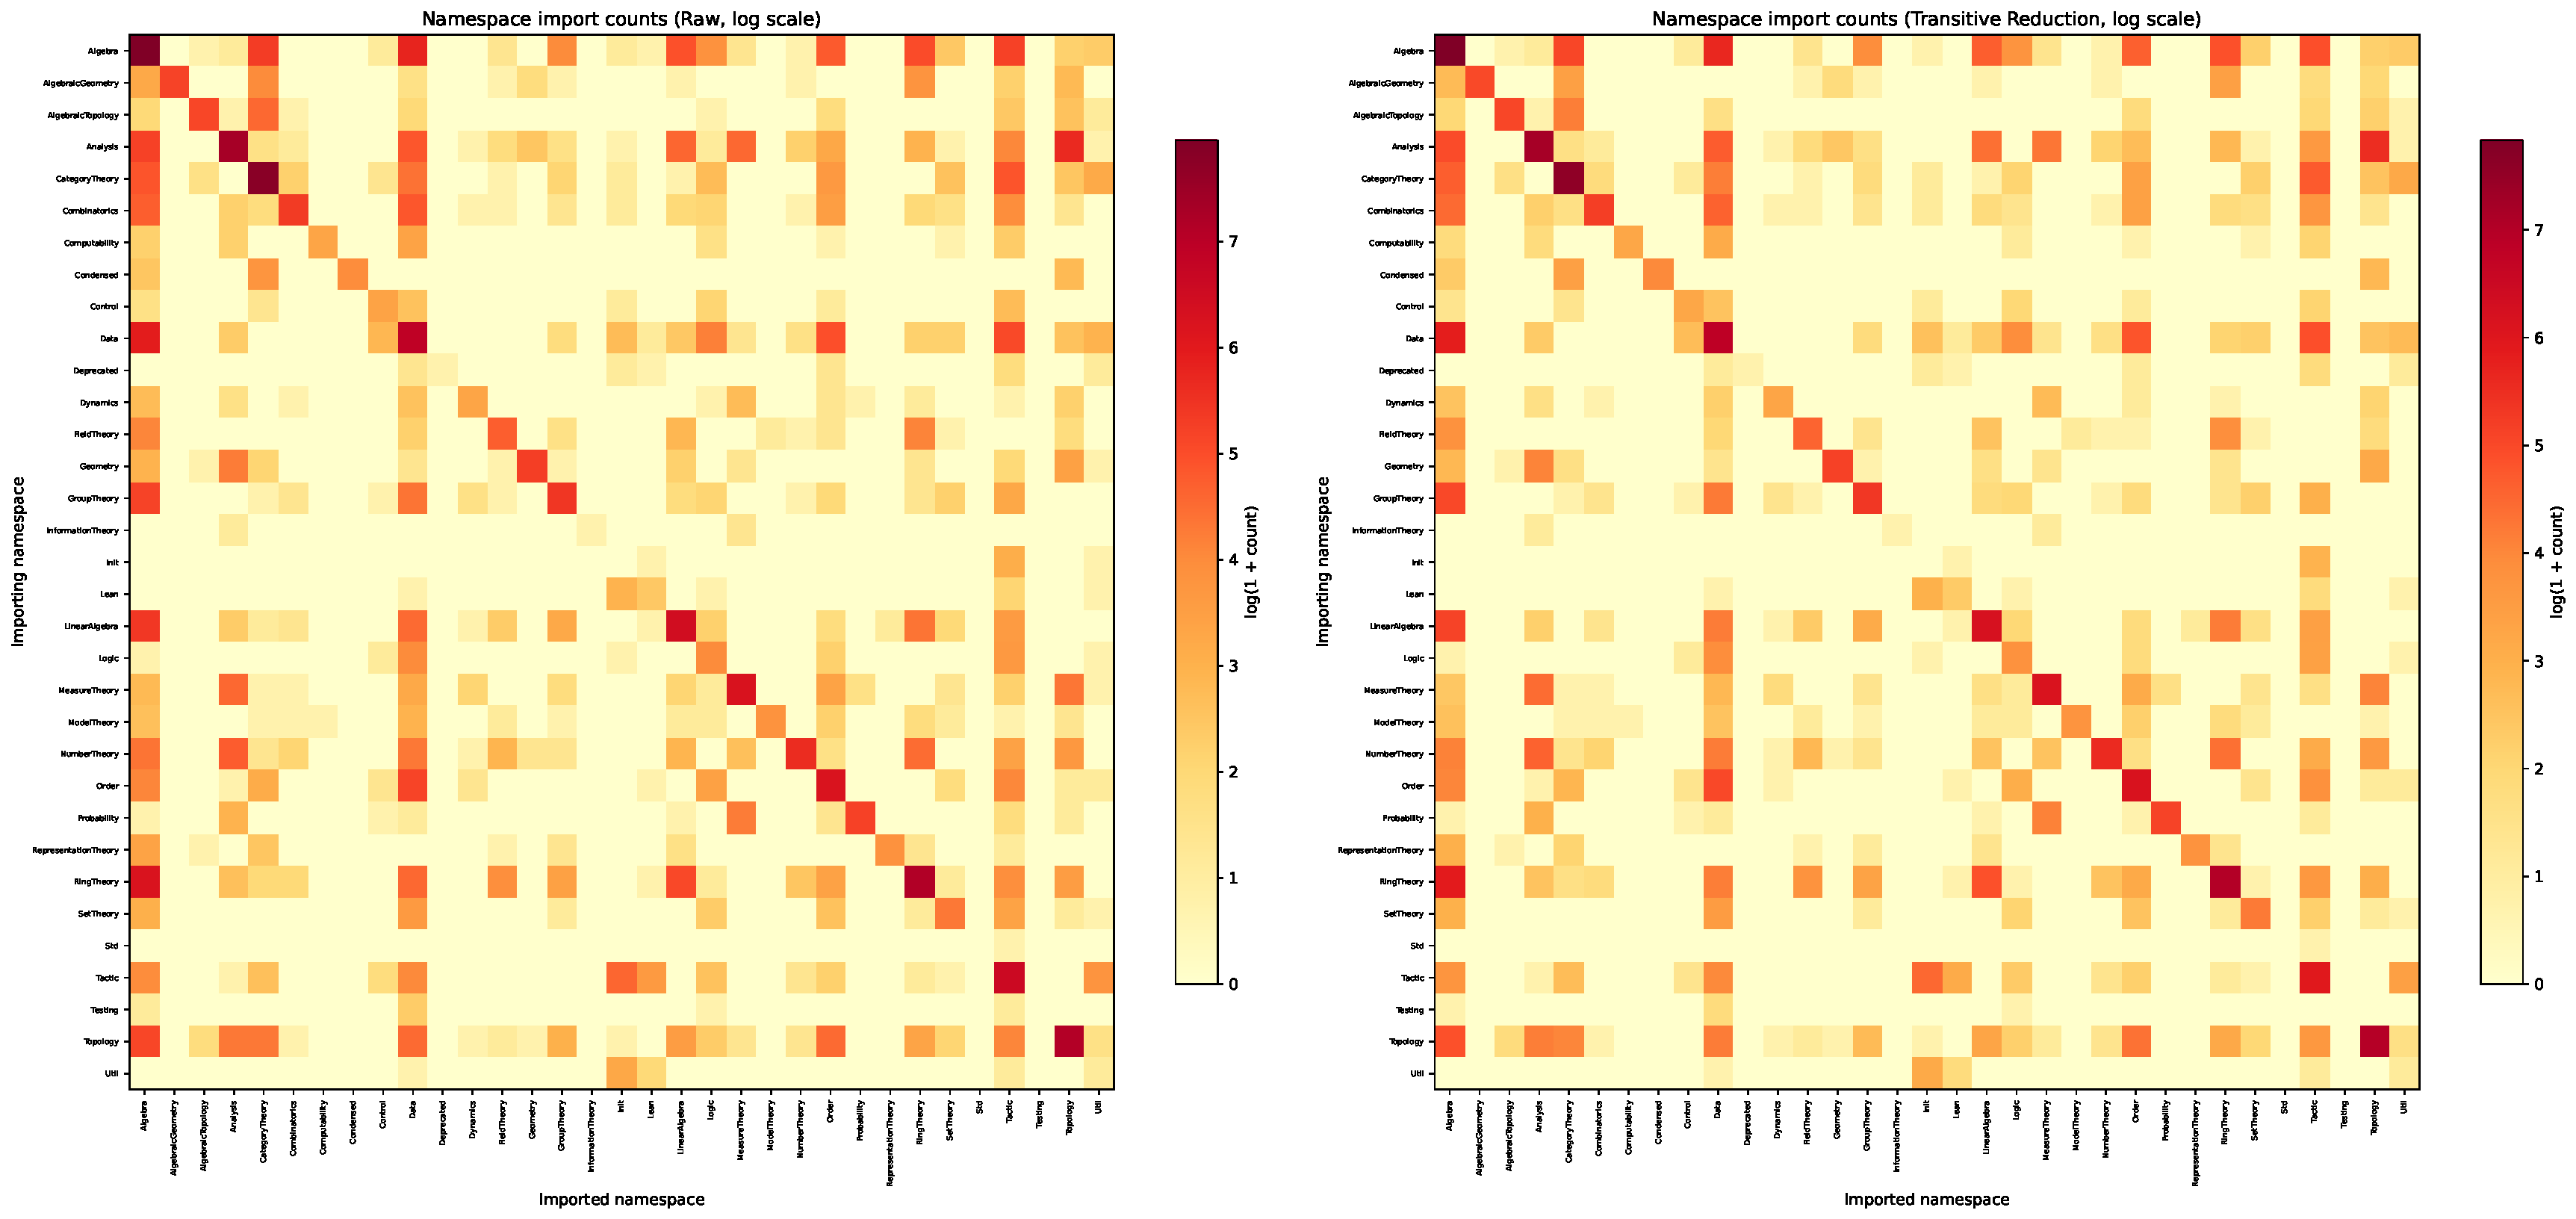
\includegraphics[width=\textwidth]{analysis/namespace_heatmap.pdf}
\caption{Import counts between top-level directories (log scale) for $G_{\mathrm{module}}$ (left) and $G_{\mathrm{module}}^{-}$ (right). Each cell $(i, j)$ counts edges from directory~$i$ (row) to directory~$j$ (column); the diagonal captures intra-directory imports. Off-diagonal bright cells reveal cross-directory dependencies that violate the cognitive classification of~$T$. The most prominent off-diagonal entries include \module{RingTheory}$\,\to\,$\module{Algebra} and the bidirectional coupling between \module{Algebra} and \module{Data}.}
\label{fig:namespace-heatmap}
\end{figure}

The strongest inter-directory dependency is \module{RingTheory} $\to$ \module{Algebra} ($485$ edges in $G_{\mathrm{module}}$), followed by \module{Data} $\to$ \module{Algebra} ($377$) and \module{Algebra} $\to$ \module{Data} ($318$). The bidirectional flow between \module{Algebra} and \module{Data} reflects their tight coupling: algebraic structures depend on basic data types, while data type lemmas often require algebraic properties. \module{Analysis} $\to$ \module{Topology} ($289$) confirms the expected mathematical dependency of analysis on topological foundations.

Degree distribution, DAG depth, centrality, and robustness analyses for the module graph are reported in \S\ref{sec:structural-analysis}.

\begin{remark}[Language contingency]
\label{rem:language-contingency}
The module graph's topology is shaped not only by mathematical dependencies but by Lean~4's specific compilation model: its prohibition of cyclic imports, its transitive visibility semantics, and the \texttt{public import} mechanism that allows selective re-export. Design choices such as fine-grained incremental compilation, selective re-export at the declaration level, or explicit interface files would alter the structure of $G_{\mathrm{module}}$ even for identical mathematical content. The structural statistics reported in this section---$17.5\%$ redundancy, $153$-layer depth, mean out-degree~$3.1$---should be understood as properties of formalized mathematics \emph{in Lean~4}, not of formalized mathematics in general.
\end{remark}

\subsection{Analysis}
\label{sec:module_conclusion}
Our structural analysis of the \module{Mathlib} module graph allows us to characterize the architecture of a large-scale formal library. We find that \module{Mathlib} does not resemble a random network or a simple hierarchy; rather, it is a \textit{deep, engineered backbone} supporting a vast, shallow application layer. These findings have three implications for the future of formal mathematical libraries.

\medskip
\noindent \textit{1. The tension between logical precision and cognitive management.} \\
The divergence between the raw module graph $G_{\mathrm{module}}$ and its transitive reduction $G_{\mathrm{module}}^{-}$ quantifies the human cost of organizing logic. The 17.5\% edge redundancy (\S\ref{sec:transitive-reduction}) is not merely inefficiency; it represents the \textit{cognitive API} of the library. Developers import entire theories (umbrella modules) to maintain mental models of the library, sacrificing logical minimality for usability. This suggests that future tools must distinguish between \textit{dependency for compilation} (minimality) and \textit{dependency for discovery} (redundancy).

Dependency for compilation follows the strict logical requirements of the type checker, ensuring that the build system avoids cycles and minimizes checking time. In contrast, dependency for discovery serves the human prover and the automation: it brings tactics, notation, and type class instances into scope, populating the context for search and elaboration. We argue that the 17.5\% redundancy observed in \module{Mathlib} is not an inefficiency but a structural feature that creates robustness against refactoring and simplifies the user interface. Optimizing solely for the transitive reduction would likely degrade the interactive experience, suggesting that future proof assistants should explicitly model these two layers separately: a minimal graph for the build system and a rich, redundant graph for the user.

\medskip
\noindent \textit{2. The architectural source of compilation bottlenecks.} \\
The layer-width profile (\S\ref{sec:dag-depth}) reveals a distinct \textit{funnel topology}: a massive leaf layer ($>1,400$ modules) resting on a deep, narrow foundation. This extreme verticality (153 layers) contrasts sharply with the flatter citation graphs of informal mathematics. While this depth ensures rigorous consistency, it creates significant structural fragility: changes in the narrow ``waist'' of the funnel (high-betweenness modules) trigger massive recompilation cascades. This identifies a critical scalability challenge: as libraries grow, the depth of the dependency chain becomes a liability that may require aggressive modularization or distinct compilation units.

Moreover, this topology imposes a distinct evolutionary pressure on the library's development. Unlike informal mathematics, where foundational texts are static references, the modules in \module{Mathlib}'s ``theoretical waist'' remain mutable code. The depth of 153 layers implies that the maintenance cost of a lemma is strictly a function of its topological depth: a change in the narrow waist invalidates the verification of thousands of downstream results. Consequently, we predict that monolithic libraries will eventually hit a \textit{critical depth threshold} where the cost of coherence checks exceeds the capacity for rapid iteration. Future architectures will likely need to break this funnel into \textit{federated tiers}---effectively freezing the foundational layers into pre-compiled artifacts---to decouple the logical necessity of depth from the operational necessity of build speed.

Our analysis captures a single snapshot (commit \texttt{534cf0b}). Whether these structural properties are stable or evolving---and whether the 17.5\% redundancy rate and 153-layer depth are increasing, stable, or approaching a critical threshold---remains an open question that longitudinal analysis across \module{Mathlib} versions must address.

\medskip
\noindent \textit{3. Centrality as a proxy for maintenance roles.} \\
We propose that the centrality measures computed in \S\ref{sec:centrality} should be interpreted as distinct maintenance signals.
\begin{itemize}
    \item \textit{In-degree} identifies the \textit{vocabulary} of the library (utilities used locally).
    \item \textit{PageRank} identifies the \textit{axiomatic core} (the deep dependencies that underpin the truth of the system).
    \item \textit{Betweenness} identifies \textit{structural bridges} (modules that connect disparate mathematical subfields).
\end{itemize}
Refactoring a high-betweenness module is riskier than refactoring a high in-degree module, as the former disrupts the connective tissue between theories.

This taxonomy offers a blueprint for automated maintenance. Currently, continuous integration systems treat all modifications with uniform computational cost, yet the \textit{structural cost} of breaking a bridge module is disproportionately higher. By embedding these centrality metrics into the review pipeline, maintainers can implement \textit{adaptive stability guarantees}: enforcing strict backward compatibility for the axiomatic core (high PageRank) and the connective bridges (high betweenness), while permitting rapid, experimental iteration on the vocabulary (high in-degree) and the leaves. This evolution toward metric-driven governance is essential to sustain the collaborative growth of a unified mathematical library, preventing it from collapsing under the maintenance burden of its own interconnected weight. From an engineering perspective, the PageRank and betweenness rankings (Table~\ref{tab:centrality}) offer a principled priority ordering for compilation optimization and CI resource allocation: modifications to high-centrality modules warrant broader downstream testing.

\medskip
These three observations---the cognitive redundancy layer, the deep funnel architecture, and the divergence of centrality roles---taken together, suggest a hypothesis about the growth mechanism of formal libraries.

\medskip
\noindent \textit{Hypothesis: The Curated Small-World.} \\
Finally, we hypothesize that successful formal libraries naturally evolve into \textit{curated small-world networks}. Unlike social networks which grow via preferential attachment, \module{Mathlib} grows via \textit{semantic attachment}: new modules cluster tightly within top-level directories (high local clustering), while deliberately placed bridge modules (high betweenness) maintain global connectivity. This structure likely represents an optimal evolutionary state for collaborative formalization, balancing the isolation needed for parallel development with the connectivity needed for a unified mathematical universe.

The fact that 100\% of modules belong to a single weakly connected component provides empirical evidence for the structural unification of mathematical theories within \module{Mathlib}. While the module tree partitions the library into distinct hierarchies, the density of inter-directory edges (37.1\%, \S\ref{sec:cross-namespace}) functions as a system of high-betweenness shortcuts that prevent the library from fracturing into isolated ``theory islands.'' Our analysis of targeted node removal (Table~\ref{tab:robustness}) demonstrates that this connectivity is remarkably resilient; as noted in Remark~\ref{rem:robustness}, over 99\% of modules remain in the giant component even after the removal of the five most central hubs. We conclude that \module{Mathlib}'s curated small-world topology is what enables foundational improvements in one domain (e.g., Algebra) to propagate efficiently to distant ones (e.g., Analysis), ensuring that the library remains a globally coherent, rather than merely modular, corpus of knowledge.

The curated small-world is the form in which the tension between $T$ and $G_{\mathrm{module}}$ reaches dynamic equilibrium---but this equilibrium is not static. The module tree $T$ actively shapes $G_{\mathrm{module}}$: developers import along the cognitive contours of $T$, producing the 62.9\% intra-directory concentration and the directional redundancy identified in \S\ref{sec:transitive-reduction}. Simultaneously, $G_{\mathrm{module}}$ reshapes $T$: the 37.1\% of edges that cross directory boundaries exert pressure on the cognitive classification, and \module{Mathlib}'s ongoing directory reorganizations---such as the gradual absorption of \module{RingTheory} into \module{Algebra}---are precisely the points where logical necessity forces cognitive categories to yield. Neither $T$ alone nor $G_{\mathrm{module}}$ alone determines the architecture; each continuously remakes the other.

This mutual determination also governs the library's evolution. The accumulation of depth (153 layers), cross-directory density (37.1\%), and hub concentration represents the growing tension between logical structure and cognitive organization. Our prediction of a critical depth threshold (\S\ref{sec:dag-depth}) is not merely an engineering forecast; it is the point at which this accumulated pressure forces a structural transformation---the restructuring of the library into federated tiers. In this sense, formalization does not dissolve the human organization of mathematics, nor does it simply reveal where that organization must yield. It initiates a feedback loop: the formal product reshapes the cognitive framework that produced it, which in turn reshapes the next generation of formal products.